\documentclass[titlepage]{report}


% Preamble

%% Packages to deal with images and links
\usepackage{graphicx}
\usepackage{float}
\usepackage{color}
\usepackage{xcolor}
\usepackage{parskip}
\usepackage[hyphens]{url}
\usepackage[hypertexnames=false, bookmarks=true, bookmarksnumbered=true, breaklinks=true, linkbordercolor={1 1 1}]{hyperref}
\usepackage{listings}
\usepackage{standalone}
%\usepackage{includex}

%% Chapter titles
\usepackage[T1]{fontenc}
\usepackage{titlesec, blindtext, color}
\definecolor{gray75}{gray}{0.75}
\newcommand{\hsp}{\hspace{20pt}}
\titleformat{\chapter}[hang]{\Huge\bfseries}{\thechapter\hsp\textcolor{gray75}{|}\hsp}{0pt}{\Huge\bfseries}

% Required packages
\usepackage{graphicx}

% Formatting options
\renewcommand{\chaptername}{}
\newcommand{\theTitle}{System And Software Architecture}
\newcommand{\filename}[1]{\texttt{#1}}

% Footnote stuff
\newcommand{\savefootnote}[2]{\footnote{\label{#1}#2}}
\newcommand{\repeatfootnote}[1]{\textsuperscript{\ref{#1}}}

\usepackage{acronym}
\acrodef{NEMA}[NEMA]{National Electrical Manufacturers Association}

% This sets up the coloring for all the included codes

\makeatletter
\def\PY@reset{\let\PY@it=\relax \let\PY@bf=\relax%
    \let\PY@ul=\relax \let\PY@tc=\relax%
    \let\PY@bc=\relax \let\PY@ff=\relax}
\def\PY@tok#1{\csname PY@tok@#1\endcsname}
\def\PY@toks#1+{\ifx\relax#1\empty\else%
    \PY@tok{#1}\expandafter\PY@toks\fi}
\def\PY@do#1{\PY@bc{\PY@tc{\PY@ul{%
    \PY@it{\PY@bf{\PY@ff{#1}}}}}}}
\def\PY#1#2{\PY@reset\PY@toks#1+\relax+\PY@do{#2}}

\expandafter\def\csname PY@tok@gd\endcsname{\def\PY@tc##1{\textcolor[rgb]{0.63,0.00,0.00}{##1}}}
\expandafter\def\csname PY@tok@gu\endcsname{\let\PY@bf=\textbf\def\PY@tc##1{\textcolor[rgb]{0.50,0.00,0.50}{##1}}}
\expandafter\def\csname PY@tok@gt\endcsname{\def\PY@tc##1{\textcolor[rgb]{0.00,0.25,0.82}{##1}}}
\expandafter\def\csname PY@tok@gs\endcsname{\let\PY@bf=\textbf}
\expandafter\def\csname PY@tok@gr\endcsname{\def\PY@tc##1{\textcolor[rgb]{1.00,0.00,0.00}{##1}}}
\expandafter\def\csname PY@tok@cm\endcsname{\let\PY@it=\textit\def\PY@tc##1{\textcolor[rgb]{0.25,0.50,0.50}{##1}}}
\expandafter\def\csname PY@tok@vg\endcsname{\def\PY@tc##1{\textcolor[rgb]{0.10,0.09,0.49}{##1}}}
\expandafter\def\csname PY@tok@m\endcsname{\def\PY@tc##1{\textcolor[rgb]{0.40,0.40,0.40}{##1}}}
\expandafter\def\csname PY@tok@mh\endcsname{\def\PY@tc##1{\textcolor[rgb]{0.40,0.40,0.40}{##1}}}
\expandafter\def\csname PY@tok@go\endcsname{\def\PY@tc##1{\textcolor[rgb]{0.50,0.50,0.50}{##1}}}
\expandafter\def\csname PY@tok@ge\endcsname{\let\PY@it=\textit}
\expandafter\def\csname PY@tok@vc\endcsname{\def\PY@tc##1{\textcolor[rgb]{0.10,0.09,0.49}{##1}}}
\expandafter\def\csname PY@tok@il\endcsname{\def\PY@tc##1{\textcolor[rgb]{0.40,0.40,0.40}{##1}}}
\expandafter\def\csname PY@tok@cs\endcsname{\let\PY@it=\textit\def\PY@tc##1{\textcolor[rgb]{0.25,0.50,0.50}{##1}}}
\expandafter\def\csname PY@tok@cp\endcsname{\def\PY@tc##1{\textcolor[rgb]{0.74,0.48,0.00}{##1}}}
\expandafter\def\csname PY@tok@gi\endcsname{\def\PY@tc##1{\textcolor[rgb]{0.00,0.63,0.00}{##1}}}
\expandafter\def\csname PY@tok@gh\endcsname{\let\PY@bf=\textbf\def\PY@tc##1{\textcolor[rgb]{0.00,0.00,0.50}{##1}}}
\expandafter\def\csname PY@tok@ni\endcsname{\let\PY@bf=\textbf\def\PY@tc##1{\textcolor[rgb]{0.60,0.60,0.60}{##1}}}
\expandafter\def\csname PY@tok@nl\endcsname{\def\PY@tc##1{\textcolor[rgb]{0.63,0.63,0.00}{##1}}}
\expandafter\def\csname PY@tok@nn\endcsname{\let\PY@bf=\textbf\def\PY@tc##1{\textcolor[rgb]{0.00,0.00,1.00}{##1}}}
\expandafter\def\csname PY@tok@no\endcsname{\def\PY@tc##1{\textcolor[rgb]{0.53,0.00,0.00}{##1}}}
\expandafter\def\csname PY@tok@na\endcsname{\def\PY@tc##1{\textcolor[rgb]{0.49,0.56,0.16}{##1}}}
\expandafter\def\csname PY@tok@nb\endcsname{\def\PY@tc##1{\textcolor[rgb]{0.00,0.50,0.00}{##1}}}
\expandafter\def\csname PY@tok@nc\endcsname{\let\PY@bf=\textbf\def\PY@tc##1{\textcolor[rgb]{0.00,0.00,1.00}{##1}}}
\expandafter\def\csname PY@tok@nd\endcsname{\def\PY@tc##1{\textcolor[rgb]{0.67,0.13,1.00}{##1}}}
\expandafter\def\csname PY@tok@ne\endcsname{\let\PY@bf=\textbf\def\PY@tc##1{\textcolor[rgb]{0.82,0.25,0.23}{##1}}}
\expandafter\def\csname PY@tok@nf\endcsname{\def\PY@tc##1{\textcolor[rgb]{0.00,0.00,1.00}{##1}}}
\expandafter\def\csname PY@tok@si\endcsname{\let\PY@bf=\textbf\def\PY@tc##1{\textcolor[rgb]{0.73,0.40,0.53}{##1}}}
\expandafter\def\csname PY@tok@s2\endcsname{\def\PY@tc##1{\textcolor[rgb]{0.73,0.13,0.13}{##1}}}
\expandafter\def\csname PY@tok@vi\endcsname{\def\PY@tc##1{\textcolor[rgb]{0.10,0.09,0.49}{##1}}}
\expandafter\def\csname PY@tok@nt\endcsname{\let\PY@bf=\textbf\def\PY@tc##1{\textcolor[rgb]{0.00,0.50,0.00}{##1}}}
\expandafter\def\csname PY@tok@nv\endcsname{\def\PY@tc##1{\textcolor[rgb]{0.10,0.09,0.49}{##1}}}
\expandafter\def\csname PY@tok@s1\endcsname{\def\PY@tc##1{\textcolor[rgb]{0.73,0.13,0.13}{##1}}}
\expandafter\def\csname PY@tok@sh\endcsname{\def\PY@tc##1{\textcolor[rgb]{0.73,0.13,0.13}{##1}}}
\expandafter\def\csname PY@tok@sc\endcsname{\def\PY@tc##1{\textcolor[rgb]{0.73,0.13,0.13}{##1}}}
\expandafter\def\csname PY@tok@sx\endcsname{\def\PY@tc##1{\textcolor[rgb]{0.00,0.50,0.00}{##1}}}
\expandafter\def\csname PY@tok@bp\endcsname{\def\PY@tc##1{\textcolor[rgb]{0.00,0.50,0.00}{##1}}}
\expandafter\def\csname PY@tok@c1\endcsname{\let\PY@it=\textit\def\PY@tc##1{\textcolor[rgb]{0.25,0.50,0.50}{##1}}}
\expandafter\def\csname PY@tok@kc\endcsname{\let\PY@bf=\textbf\def\PY@tc##1{\textcolor[rgb]{0.00,0.50,0.00}{##1}}}
\expandafter\def\csname PY@tok@c\endcsname{\let\PY@it=\textit\def\PY@tc##1{\textcolor[rgb]{0.25,0.50,0.50}{##1}}}
\expandafter\def\csname PY@tok@mf\endcsname{\def\PY@tc##1{\textcolor[rgb]{0.40,0.40,0.40}{##1}}}
\expandafter\def\csname PY@tok@err\endcsname{\def\PY@bc##1{\setlength{\fboxsep}{0pt}\fcolorbox[rgb]{1.00,0.00,0.00}{1,1,1}{\strut ##1}}}
\expandafter\def\csname PY@tok@kd\endcsname{\let\PY@bf=\textbf\def\PY@tc##1{\textcolor[rgb]{0.00,0.50,0.00}{##1}}}
\expandafter\def\csname PY@tok@ss\endcsname{\def\PY@tc##1{\textcolor[rgb]{0.10,0.09,0.49}{##1}}}
\expandafter\def\csname PY@tok@sr\endcsname{\def\PY@tc##1{\textcolor[rgb]{0.73,0.40,0.53}{##1}}}
\expandafter\def\csname PY@tok@mo\endcsname{\def\PY@tc##1{\textcolor[rgb]{0.40,0.40,0.40}{##1}}}
\expandafter\def\csname PY@tok@kn\endcsname{\let\PY@bf=\textbf\def\PY@tc##1{\textcolor[rgb]{0.00,0.50,0.00}{##1}}}
\expandafter\def\csname PY@tok@mi\endcsname{\def\PY@tc##1{\textcolor[rgb]{0.40,0.40,0.40}{##1}}}
\expandafter\def\csname PY@tok@gp\endcsname{\let\PY@bf=\textbf\def\PY@tc##1{\textcolor[rgb]{0.00,0.00,0.50}{##1}}}
\expandafter\def\csname PY@tok@o\endcsname{\def\PY@tc##1{\textcolor[rgb]{0.40,0.40,0.40}{##1}}}
\expandafter\def\csname PY@tok@kr\endcsname{\let\PY@bf=\textbf\def\PY@tc##1{\textcolor[rgb]{0.00,0.50,0.00}{##1}}}
\expandafter\def\csname PY@tok@s\endcsname{\def\PY@tc##1{\textcolor[rgb]{0.73,0.13,0.13}{##1}}}
\expandafter\def\csname PY@tok@kp\endcsname{\def\PY@tc##1{\textcolor[rgb]{0.00,0.50,0.00}{##1}}}
\expandafter\def\csname PY@tok@w\endcsname{\def\PY@tc##1{\textcolor[rgb]{0.73,0.73,0.73}{##1}}}
\expandafter\def\csname PY@tok@kt\endcsname{\def\PY@tc##1{\textcolor[rgb]{0.69,0.00,0.25}{##1}}}
\expandafter\def\csname PY@tok@ow\endcsname{\let\PY@bf=\textbf\def\PY@tc##1{\textcolor[rgb]{0.67,0.13,1.00}{##1}}}
\expandafter\def\csname PY@tok@sb\endcsname{\def\PY@tc##1{\textcolor[rgb]{0.73,0.13,0.13}{##1}}}
\expandafter\def\csname PY@tok@k\endcsname{\let\PY@bf=\textbf\def\PY@tc##1{\textcolor[rgb]{0.00,0.50,0.00}{##1}}}
\expandafter\def\csname PY@tok@se\endcsname{\let\PY@bf=\textbf\def\PY@tc##1{\textcolor[rgb]{0.73,0.40,0.13}{##1}}}
\expandafter\def\csname PY@tok@sd\endcsname{\let\PY@it=\textit\def\PY@tc##1{\textcolor[rgb]{0.73,0.13,0.13}{##1}}}

\def\PYZbs{\char`\\}
\def\PYZus{\char`\_}
\def\PYZob{\char`\{}
\def\PYZcb{\char`\}}
\def\PYZca{\char`\^}
\def\PYZam{\char`\&}
\def\PYZlt{\char`\<}
\def\PYZgt{\char`\>}
\def\PYZsh{\char`\#}
\def\PYZpc{\char`\%}
\def\PYZdl{\char`\$}
\def\PYZti{\char`\~}
% for compatibility with earlier versions
\def\PYZat{@}
\def\PYZlb{[}
\def\PYZrb{]}
\makeatother


% And this labels it nicely
\usepackage{caption}
\DeclareCaptionFont{white}{\color{white}}
\DeclareCaptionFormat{listing}{\colorbox{gray}{\parbox{\textwidth}{#1#2#3}}}
\captionsetup[table]{format=listing,labelfont=white,textfont=white}


\begin{document}

% Title and authors
\title{POW-R Low Level Design Document}
\author{
  Grace De Geus\\
  \texttt{gdegeus@vtc.edu}
  \and
  Charles Hathaway\\
  \texttt{chathaway2@vtc.edu}
  \and
  Nate Pickett\\
  \texttt{npickett@vtc.edu}
  \and
  Niloc Quimby\\
  \texttt{nquimby@vtc.edu}
  \and
  Forest Immel\\
  \texttt{fimmel@vtc.edu}
}
\maketitle



\setcounter{page}{1}
\pagenumbering{roman}

% Table of contents
\tableofcontents
\newpage


\listoffigures
\textbf{\addcontentsline{toc}{chapter}{List of Figures}}
\newpage

\listoftables
\textbf{\addcontentsline{toc}{chapter}{List of Tables}}
\newpage

\setcounter{page}{1}
\pagenumbering{arabic}

% Introduction and some basic things
\chapter{Introduction}

\section{Purpose of this Document}
This document describes the low level design of all components of the \ac{POW-R} system.
The purpose of the  Design Document is to provide a description of the design of a system
fully enough to allow for software development to proceed with an understanding of what is to be
built and how it is expected to built.  This document provides information
necessary to provide description of the details for the software and system to be built.

\section{Scope}
This Design Document is for a base level system which will work as a proof of concept for
the use of building a system the provides a base level of functionality to show feasibility for large
scale production use.  This Design is focused on the base level system and critical parts
of the system.




% Hardware design
%% Template file for all Software/Hardware modules

% Replace "Name of Module" with the name of this module
\chapter{Hardware Design Overview}

\section{Description}

The POW-R project is comprised of two main hardware components, the Server and the Satellites. 
The Server refers to the physical hardware from which the Display shall be served. 
It also acts as the data center for all Satellites associated to it, collecting data and storing it in a hard drive. 
The Satellites will talk over ZigBee specification to the one Zigbee module connected to the Server. 
That one Zigbee module can talk to the Server over Universal Serial Bus (USB).
 
Figure \ref{SystemOverview} shows the layout of the hardware system.

\begin{figure}[H]
\centering
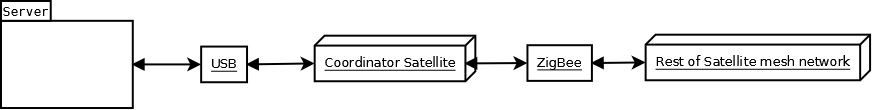
\includegraphics[scale=0.3]{Hardware/images/SystemOverview.png}
\caption{System Overview}
\label{SystemOverview}
\end{figure}

\section{The Server}
%% Template file for all Hardware modules

% Replace "Name of Module" with the name of this module
\subsection{PC Hardware}

\subsubsection{Mainboard}
The Server's main hardware component is the mainboard, a SYS9400-ECX Developer-Ready Reference Platform. 
It's a small form-factor, low-power machine with the following specs:

\begin{itemize}
	\item 1.6 GHz Intel Atom E6XX Series Processor
	\item 1 GB DDR2 RAM
	\item Roughly 6" by 4"
	\item Various connection interfaces:
	\begin{itemize}
		\item 2x SATA ports
		\item Header for Solid State Drive (SSD) power
		\item Ethernet port
		\item 5x USB 2.0 ports
		\item General Purpose Input/Output (GPIO) pin header
	\end{itemize}
\end{itemize}

\subsubsection{Potential Problems}
If for whatever reason using this mainboard falls through: 
It should be noted that the requirements for the Server hardware concern not just specifications, but interfaces as well.
In particular, this project requires at least Ethernet, 2 USB ports, a SATA port, and accessible GPIO pins.
\subsubsection{Storage}
The Server's mainboard is connected via SATA to a 40GB SSD.

\subsubsection{Power Supply}
An adapter rated for 12VDC @ 3A is used to connect the Server's board to mains electricity.

%% Template file for all Software/Hardware modules

\subsection{Add-Ons}
The Server provides for the computational needs of the POW-R project; 
More hardware shall be added before the utility needs of the project are met.

\subsubsection{IP Display}
The IP of the Server shall be displayed somewhere on it's casing. 
The user will enter this IP into their browser to access the Display.

This will be achieved by connecting an Arduino via USB to the Server, and housing it inside the Server's casing. 
The Arduino will be connected to an LCD display which will output the network IP of the Server. 
Figure \ref{ArduinoLCD} shows the interaction between Server and Arduino.

\begin{figure}
\centering
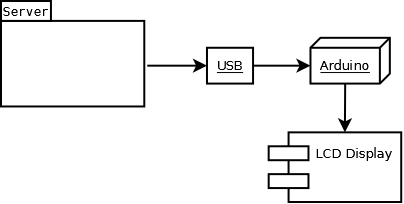
\includegraphics[scale=0.5]{Hardware/images/ArduinoLCD.png}
\caption{IP Display Diagram}
\label{ArduinoLCD}
\end{figure}

The IP of the system can be obtained via kernel module, and sent to the Arduino one byte at a time. 
This works well, since the Arduino connects over serial and thusly takes a byte at a time.

\subsection{GPIO Pins}
As mentioned above in the "PC Hardware" section, the mainboard is outfitted with a GPIO pin header. 
A Linux distribution will be used for the Server's operating system, which must support interaction with such pins. 

A folder can be found in the Linux kernel, at the location \filename{/sys/class/gpio} that helps with GPIO manipulation. 
To set up a single GPIO pin, one must type the following command into a terminal (as root):

\begin{lstlisting}
	$ echo N > /sys/class/gpio/export
	(where N must be a GPIO pin number)
\end{lstlisting}

When this command is issued, a directory is made inside the \filename{gpio} directory, named \filename{gpioN}, where N is the GPIO pin number you passed. 
Two files will be in that new directory, \filename{direction} and \filename{value}. 
\filename{direction} can only contain "in" or "out" with no leading characters, spaces, line breaks, etc.
\filename{value} can only contain "1" or "0" and can be read or written to at any time.
These files, \filename{direction} and \filename{value} are responsible for what kind of pin it is (input or output) and what the current value is (1 or 0), respectively.

NOTE: The pin number you must echo into \filename{/sys/class/gpio/export} is not necessarily the number of the actual pin on the board, but may refer to the pin of the bridge that connects the GPIO port to the motherboard.

The subsections below are buttons that the Server must have, and each of these buttons connects to a GPIO pin.


\subsubsection{Power Switch}
A standard rocker switch will be added to the case to provide the user with a way to turn the Server on and off. 
The style of the switch will clearly signify "On" or "Off".

\subsubsection{Factory Reset\repeatfootnote{opt}}
This button should intentionally be placed somewhere inconvenient: 
Sunken into the case far enough that you need a skinny rod (such as a paperclip) to push it, and in a spot
that chaotic forces (children, mean people, God's divine will) will not notice it.

\subsubsection{Connect to Satellite}
A button will be added to the Server that allows a user to add a Satellite easily.
When a user wants to add a Satellite to the network, the following series of events should take place, in order:

\begin{itemize}
	\item User plugs Satellite into wall outlet
	\item User presses "connect" button on Satellite
	\item User presses "connect" button on Server
	\item Satellite is now connected
\end{itemize}
	
\subsection{Server Hull}
The Server needs a protective casing, for several reasons. 
On the physical level, a durable casing will protect the hardware. 
The casing also serves to render unnecessary ports inaccessible to users. 
Lastly, the casing is important in the sense that the term "Server" currently only applies to the mainboard, 
and most people think of a legitimate Server as something physical, encased in a box, that's protected and hidden away, exactly as a Server should be.

As far as prototyping goes, the casing can be as simple as a folded piece of aluminum
with holes cut in it to fit the IP display, the buttons, and any ports that must be
exposed. As an end-game product, the casing would probably be a little less "junkyard."

\input{Hardware/Server-TalkToXbee}
\subsection{Potential Problems}
As of right now, the Server has not been explored, and as with the rest of this project, is unfamiliar territory. 


\section{The Satellites}
The Satellites are made up of two sets of hardware: 
Instruments for measuring current and voltage, and radios for communicating that data to the Server. 
The end product shall have a hard casing around it, NEMA 5-15 sockets on one side, and prongs for a NEMA 5-15 male end on the other. 
However, it should be noted that prototyping will most likely involve all of the hardware being spread out on breadboards.
%% Template file for all Software/Hardware modules

% Replace "Name of Module" with the name of this module
\subsection{Measurement Hardware}
Current and voltage running through the mains outlet to the Satellite's associated device must be measured and sent to the Server. 

%% Template file for all Software/Hardware modules

\subsection{Communications Hardware}

% Describe hardware setup for our
% XBee modules

For the communication between the Server and the Satellites,
we will be using the Xbee Series 2 Radio Modules.

\subsubsection{XBee Series 2 Radio Modules}

% Might want to mention we want series 2 for
% Zigbee, but ZigBee has it's own module since
% it's a fairly large part of this design

\subsubsection{Interface Board}

% This section is a little vague at the moment.
% Currently we're using Digi Interface Boards,
% but we may need to move to an Arduino if these
% boards lack an A/D converter pin. Haven't
% looked into it yet. In either case, whatever
% interface board we use will connect the
% measuring circuit to the radio. Might
% need diagram for this.

%% Template file for all Software/Hardware modules

\subsection{ZigBee Standard}
ZigBee is a standard that uses 802.15.4 wireless protocol as it's foundation. It's 
particularly useful for setting up ad-hoc mesh networks. Much like how any Bluetooth
devices can talk to each other, any ZigBee devices nearby can talk to each other (so 
long as they have the proper permissions).

\subsubsection{Why ZigBee?}
The advantage of using ZigBee is that it lines up with the requirements of the POW-R
project. It's a specification targeted for low-power, low-data applications that need
to be secure. 

Another advantage of using ZigBee is that XBee radios, which also fit the requirements
of the POW-R project, are ZigBee-compliant, so the forming of a mesh network can happen
quickly and easily.

\subsubsection{Device Types}
The nodes of a ZigBee network are obviously ZigBee devices, but from the network's
perspective, there are three distinct types of ZigBee device:

\begin{itemize}
	\item Coordinator
	\item Router
	\item End Device
\end{itemize}

The coordinator runs the network, keeps it healthy, makes sure everybody is talking when
they should be, and overall, just maintains the Mesh. It is also the device that is 
typically plugged into a computer via USB or some other serial interface, meaning
that this is the node you want to send data to. There cannot be a ZigBee network
without exactly one coordinator.

Routers are fully functional ZigBee modules, capable of taking care of themselves and
routing messages across the Mesh. Routers are capable of being "parent" devices.

End devices are low-power ZigBee devices that don't do any routing. They can only talk
to one other device, which is referred to as it's "parent" device. A router or a coordinator
may be a parent device, but not another end device.

In the POW-R project, the coordinator will be attached to the Server so that it may
also act as a data bridge between the Server and the Satellites. The rest of the 
Satellites are routers; There will be no end devices in the POW-R's mesh network.


\subsubsection{Network Topology}
Zigbee supports four network topologies, shown in Figure \ref{NetTopo}. A ZigBee network
is defined by two rules:

\begin{itemize}
	\item A ZigBee network must have two or more ZigBee devices
	\item One of those devices \emph{must} be a coordinator
\end{itemize}

As mentioned before, the POW-R project will use the Mesh configuration, but without end 
devices. This means that the Mesh will consist entirely of routers and one coordinator.

\begin{figure}
\centering
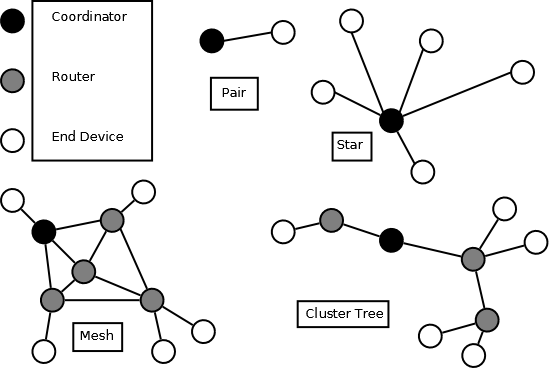
\includegraphics[scale=0.3]{Hardware/images/ZigBeeNetworkTypes.png}
\caption{ZigBee Network Topologies}
\label{NetTopo}
\end{figure}
\subsection{Potential Problems}
XBee Series 2 radios and their interface boards have as of yet been unexplored. 
This means that as with the rest of this project, there will be about as much learning as there will be doing. 
To counteract this somewhat, the engineers in charge of weaving the Mesh have learning materials that are perfect for this project. 

% Software design
%% Template file for all Software/Hardware modules

% Replace "Name of Module" with the name of this module
\chapter{Hardware Design Overview}

\section{Description}

The POW-R project is comprised of two main hardware components, the Server and the Satellites. 
The Server refers to the physical hardware from which the Display shall be served. 
It also acts as the data center for all Satellites associated to it, collecting data and storing it in a hard drive. 
The Satellites will talk over ZigBee specification to the one Zigbee module connected to the Server. 
That one Zigbee module can talk to the Server over Universal Serial Bus (USB).
 
Figure \ref{SystemOverview} shows the layout of the hardware system.

\begin{figure}[H]
\centering
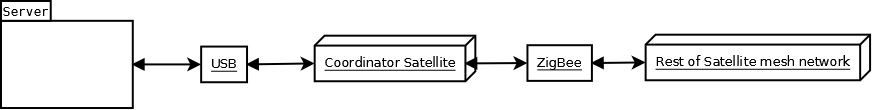
\includegraphics[scale=0.3]{Hardware/images/SystemOverview.png}
\caption{System Overview}
\label{SystemOverview}
\end{figure}

\section{The Server}
%% Template file for all Hardware modules

% Replace "Name of Module" with the name of this module
\subsection{PC Hardware}

\subsubsection{Mainboard}
The Server's main hardware component is the mainboard, a SYS9400-ECX Developer-Ready Reference Platform. 
It's a small form-factor, low-power machine with the following specs:

\begin{itemize}
	\item 1.6 GHz Intel Atom E6XX Series Processor
	\item 1 GB DDR2 RAM
	\item Roughly 6" by 4"
	\item Various connection interfaces:
	\begin{itemize}
		\item 2x SATA ports
		\item Header for Solid State Drive (SSD) power
		\item Ethernet port
		\item 5x USB 2.0 ports
		\item General Purpose Input/Output (GPIO) pin header
	\end{itemize}
\end{itemize}

\subsubsection{Potential Problems}
If for whatever reason using this mainboard falls through: 
It should be noted that the requirements for the Server hardware concern not just specifications, but interfaces as well.
In particular, this project requires at least Ethernet, 2 USB ports, a SATA port, and accessible GPIO pins.
\subsubsection{Storage}
The Server's mainboard is connected via SATA to a 40GB SSD.

\subsubsection{Power Supply}
An adapter rated for 12VDC @ 3A is used to connect the Server's board to mains electricity.

%% Template file for all Software/Hardware modules

\subsection{Add-Ons}
The Server provides for the computational needs of the POW-R project; 
More hardware shall be added before the utility needs of the project are met.

\subsubsection{IP Display}
The IP of the Server shall be displayed somewhere on it's casing. 
The user will enter this IP into their browser to access the Display.

This will be achieved by connecting an Arduino via USB to the Server, and housing it inside the Server's casing. 
The Arduino will be connected to an LCD display which will output the network IP of the Server. 
Figure \ref{ArduinoLCD} shows the interaction between Server and Arduino.

\begin{figure}
\centering
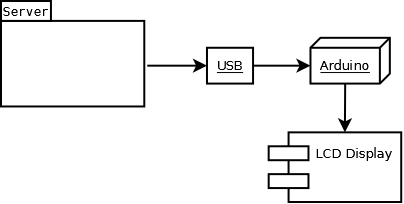
\includegraphics[scale=0.5]{Hardware/images/ArduinoLCD.png}
\caption{IP Display Diagram}
\label{ArduinoLCD}
\end{figure}

The IP of the system can be obtained via kernel module, and sent to the Arduino one byte at a time. 
This works well, since the Arduino connects over serial and thusly takes a byte at a time.

\subsection{GPIO Pins}
As mentioned above in the "PC Hardware" section, the mainboard is outfitted with a GPIO pin header. 
A Linux distribution will be used for the Server's operating system, which must support interaction with such pins. 

A folder can be found in the Linux kernel, at the location \filename{/sys/class/gpio} that helps with GPIO manipulation. 
To set up a single GPIO pin, one must type the following command into a terminal (as root):

\begin{lstlisting}
	$ echo N > /sys/class/gpio/export
	(where N must be a GPIO pin number)
\end{lstlisting}

When this command is issued, a directory is made inside the \filename{gpio} directory, named \filename{gpioN}, where N is the GPIO pin number you passed. 
Two files will be in that new directory, \filename{direction} and \filename{value}. 
\filename{direction} can only contain "in" or "out" with no leading characters, spaces, line breaks, etc.
\filename{value} can only contain "1" or "0" and can be read or written to at any time.
These files, \filename{direction} and \filename{value} are responsible for what kind of pin it is (input or output) and what the current value is (1 or 0), respectively.

NOTE: The pin number you must echo into \filename{/sys/class/gpio/export} is not necessarily the number of the actual pin on the board, but may refer to the pin of the bridge that connects the GPIO port to the motherboard.

The subsections below are buttons that the Server must have, and each of these buttons connects to a GPIO pin.


\subsubsection{Power Switch}
A standard rocker switch will be added to the case to provide the user with a way to turn the Server on and off. 
The style of the switch will clearly signify "On" or "Off".

\subsubsection{Factory Reset\repeatfootnote{opt}}
This button should intentionally be placed somewhere inconvenient: 
Sunken into the case far enough that you need a skinny rod (such as a paperclip) to push it, and in a spot
that chaotic forces (children, mean people, God's divine will) will not notice it.

\subsubsection{Connect to Satellite}
A button will be added to the Server that allows a user to add a Satellite easily.
When a user wants to add a Satellite to the network, the following series of events should take place, in order:

\begin{itemize}
	\item User plugs Satellite into wall outlet
	\item User presses "connect" button on Satellite
	\item User presses "connect" button on Server
	\item Satellite is now connected
\end{itemize}
	
\subsection{Server Hull}
The Server needs a protective casing, for several reasons. 
On the physical level, a durable casing will protect the hardware. 
The casing also serves to render unnecessary ports inaccessible to users. 
Lastly, the casing is important in the sense that the term "Server" currently only applies to the mainboard, 
and most people think of a legitimate Server as something physical, encased in a box, that's protected and hidden away, exactly as a Server should be.

As far as prototyping goes, the casing can be as simple as a folded piece of aluminum
with holes cut in it to fit the IP display, the buttons, and any ports that must be
exposed. As an end-game product, the casing would probably be a little less "junkyard."

\input{Hardware/Server-TalkToXbee}
\subsection{Potential Problems}
As of right now, the Server has not been explored, and as with the rest of this project, is unfamiliar territory. 


\section{The Satellites}
The Satellites are made up of two sets of hardware: 
Instruments for measuring current and voltage, and radios for communicating that data to the Server. 
The end product shall have a hard casing around it, NEMA 5-15 sockets on one side, and prongs for a NEMA 5-15 male end on the other. 
However, it should be noted that prototyping will most likely involve all of the hardware being spread out on breadboards.
%% Template file for all Software/Hardware modules

% Replace "Name of Module" with the name of this module
\subsection{Measurement Hardware}
Current and voltage running through the mains outlet to the Satellite's associated device must be measured and sent to the Server. 

%% Template file for all Software/Hardware modules

\subsection{Communications Hardware}

% Describe hardware setup for our
% XBee modules

For the communication between the Server and the Satellites,
we will be using the Xbee Series 2 Radio Modules.

\subsubsection{XBee Series 2 Radio Modules}

% Might want to mention we want series 2 for
% Zigbee, but ZigBee has it's own module since
% it's a fairly large part of this design

\subsubsection{Interface Board}

% This section is a little vague at the moment.
% Currently we're using Digi Interface Boards,
% but we may need to move to an Arduino if these
% boards lack an A/D converter pin. Haven't
% looked into it yet. In either case, whatever
% interface board we use will connect the
% measuring circuit to the radio. Might
% need diagram for this.

%% Template file for all Software/Hardware modules

\subsection{ZigBee Standard}
ZigBee is a standard that uses 802.15.4 wireless protocol as it's foundation. It's 
particularly useful for setting up ad-hoc mesh networks. Much like how any Bluetooth
devices can talk to each other, any ZigBee devices nearby can talk to each other (so 
long as they have the proper permissions).

\subsubsection{Why ZigBee?}
The advantage of using ZigBee is that it lines up with the requirements of the POW-R
project. It's a specification targeted for low-power, low-data applications that need
to be secure. 

Another advantage of using ZigBee is that XBee radios, which also fit the requirements
of the POW-R project, are ZigBee-compliant, so the forming of a mesh network can happen
quickly and easily.

\subsubsection{Device Types}
The nodes of a ZigBee network are obviously ZigBee devices, but from the network's
perspective, there are three distinct types of ZigBee device:

\begin{itemize}
	\item Coordinator
	\item Router
	\item End Device
\end{itemize}

The coordinator runs the network, keeps it healthy, makes sure everybody is talking when
they should be, and overall, just maintains the Mesh. It is also the device that is 
typically plugged into a computer via USB or some other serial interface, meaning
that this is the node you want to send data to. There cannot be a ZigBee network
without exactly one coordinator.

Routers are fully functional ZigBee modules, capable of taking care of themselves and
routing messages across the Mesh. Routers are capable of being "parent" devices.

End devices are low-power ZigBee devices that don't do any routing. They can only talk
to one other device, which is referred to as it's "parent" device. A router or a coordinator
may be a parent device, but not another end device.

In the POW-R project, the coordinator will be attached to the Server so that it may
also act as a data bridge between the Server and the Satellites. The rest of the 
Satellites are routers; There will be no end devices in the POW-R's mesh network.


\subsubsection{Network Topology}
Zigbee supports four network topologies, shown in Figure \ref{NetTopo}. A ZigBee network
is defined by two rules:

\begin{itemize}
	\item A ZigBee network must have two or more ZigBee devices
	\item One of those devices \emph{must} be a coordinator
\end{itemize}

As mentioned before, the POW-R project will use the Mesh configuration, but without end 
devices. This means that the Mesh will consist entirely of routers and one coordinator.

\begin{figure}
\centering
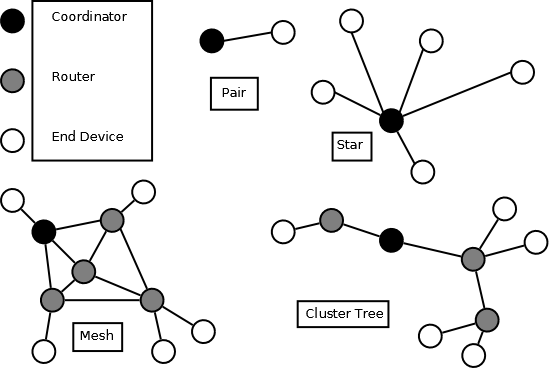
\includegraphics[scale=0.3]{Hardware/images/ZigBeeNetworkTypes.png}
\caption{ZigBee Network Topologies}
\label{NetTopo}
\end{figure}
\subsection{Potential Problems}
XBee Series 2 radios and their interface boards have as of yet been unexplored. 
This means that as with the rest of this project, there will be about as much learning as there will be doing. 
To counteract this somewhat, the engineers in charge of weaving the Mesh have learning materials that are perfect for this project. 

\newpage
%Use Cases
%% Template file for all Software/Hardware modules

% Replace "Name of Module" with the name of this module
\chapter{Hardware Design Overview}

\section{Description}

The POW-R project is comprised of two main hardware components, the Server and the Satellites. 
The Server refers to the physical hardware from which the Display shall be served. 
It also acts as the data center for all Satellites associated to it, collecting data and storing it in a hard drive. 
The Satellites will talk over ZigBee specification to the one Zigbee module connected to the Server. 
That one Zigbee module can talk to the Server over Universal Serial Bus (USB).
 
Figure \ref{SystemOverview} shows the layout of the hardware system.

\begin{figure}[H]
\centering
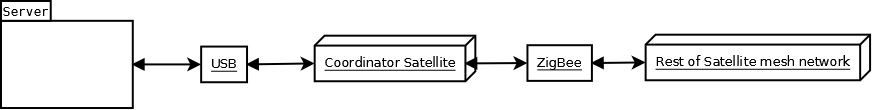
\includegraphics[scale=0.3]{Hardware/images/SystemOverview.png}
\caption{System Overview}
\label{SystemOverview}
\end{figure}

\section{The Server}
%% Template file for all Hardware modules

% Replace "Name of Module" with the name of this module
\subsection{PC Hardware}

\subsubsection{Mainboard}
The Server's main hardware component is the mainboard, a SYS9400-ECX Developer-Ready Reference Platform. 
It's a small form-factor, low-power machine with the following specs:

\begin{itemize}
	\item 1.6 GHz Intel Atom E6XX Series Processor
	\item 1 GB DDR2 RAM
	\item Roughly 6" by 4"
	\item Various connection interfaces:
	\begin{itemize}
		\item 2x SATA ports
		\item Header for Solid State Drive (SSD) power
		\item Ethernet port
		\item 5x USB 2.0 ports
		\item General Purpose Input/Output (GPIO) pin header
	\end{itemize}
\end{itemize}

\subsubsection{Potential Problems}
If for whatever reason using this mainboard falls through: 
It should be noted that the requirements for the Server hardware concern not just specifications, but interfaces as well.
In particular, this project requires at least Ethernet, 2 USB ports, a SATA port, and accessible GPIO pins.
\subsubsection{Storage}
The Server's mainboard is connected via SATA to a 40GB SSD.

\subsubsection{Power Supply}
An adapter rated for 12VDC @ 3A is used to connect the Server's board to mains electricity.

%% Template file for all Software/Hardware modules

\subsection{Add-Ons}
The Server provides for the computational needs of the POW-R project; 
More hardware shall be added before the utility needs of the project are met.

\subsubsection{IP Display}
The IP of the Server shall be displayed somewhere on it's casing. 
The user will enter this IP into their browser to access the Display.

This will be achieved by connecting an Arduino via USB to the Server, and housing it inside the Server's casing. 
The Arduino will be connected to an LCD display which will output the network IP of the Server. 
Figure \ref{ArduinoLCD} shows the interaction between Server and Arduino.

\begin{figure}
\centering
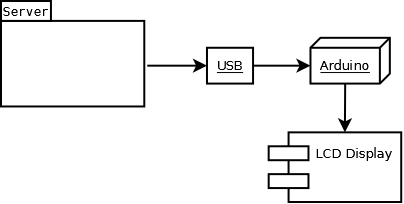
\includegraphics[scale=0.5]{Hardware/images/ArduinoLCD.png}
\caption{IP Display Diagram}
\label{ArduinoLCD}
\end{figure}

The IP of the system can be obtained via kernel module, and sent to the Arduino one byte at a time. 
This works well, since the Arduino connects over serial and thusly takes a byte at a time.

\subsection{GPIO Pins}
As mentioned above in the "PC Hardware" section, the mainboard is outfitted with a GPIO pin header. 
A Linux distribution will be used for the Server's operating system, which must support interaction with such pins. 

A folder can be found in the Linux kernel, at the location \filename{/sys/class/gpio} that helps with GPIO manipulation. 
To set up a single GPIO pin, one must type the following command into a terminal (as root):

\begin{lstlisting}
	$ echo N > /sys/class/gpio/export
	(where N must be a GPIO pin number)
\end{lstlisting}

When this command is issued, a directory is made inside the \filename{gpio} directory, named \filename{gpioN}, where N is the GPIO pin number you passed. 
Two files will be in that new directory, \filename{direction} and \filename{value}. 
\filename{direction} can only contain "in" or "out" with no leading characters, spaces, line breaks, etc.
\filename{value} can only contain "1" or "0" and can be read or written to at any time.
These files, \filename{direction} and \filename{value} are responsible for what kind of pin it is (input or output) and what the current value is (1 or 0), respectively.

NOTE: The pin number you must echo into \filename{/sys/class/gpio/export} is not necessarily the number of the actual pin on the board, but may refer to the pin of the bridge that connects the GPIO port to the motherboard.

The subsections below are buttons that the Server must have, and each of these buttons connects to a GPIO pin.


\subsubsection{Power Switch}
A standard rocker switch will be added to the case to provide the user with a way to turn the Server on and off. 
The style of the switch will clearly signify "On" or "Off".

\subsubsection{Factory Reset\repeatfootnote{opt}}
This button should intentionally be placed somewhere inconvenient: 
Sunken into the case far enough that you need a skinny rod (such as a paperclip) to push it, and in a spot
that chaotic forces (children, mean people, God's divine will) will not notice it.

\subsubsection{Connect to Satellite}
A button will be added to the Server that allows a user to add a Satellite easily.
When a user wants to add a Satellite to the network, the following series of events should take place, in order:

\begin{itemize}
	\item User plugs Satellite into wall outlet
	\item User presses "connect" button on Satellite
	\item User presses "connect" button on Server
	\item Satellite is now connected
\end{itemize}
	
\subsection{Server Hull}
The Server needs a protective casing, for several reasons. 
On the physical level, a durable casing will protect the hardware. 
The casing also serves to render unnecessary ports inaccessible to users. 
Lastly, the casing is important in the sense that the term "Server" currently only applies to the mainboard, 
and most people think of a legitimate Server as something physical, encased in a box, that's protected and hidden away, exactly as a Server should be.

As far as prototyping goes, the casing can be as simple as a folded piece of aluminum
with holes cut in it to fit the IP display, the buttons, and any ports that must be
exposed. As an end-game product, the casing would probably be a little less "junkyard."

\input{Hardware/Server-TalkToXbee}
\subsection{Potential Problems}
As of right now, the Server has not been explored, and as with the rest of this project, is unfamiliar territory. 


\section{The Satellites}
The Satellites are made up of two sets of hardware: 
Instruments for measuring current and voltage, and radios for communicating that data to the Server. 
The end product shall have a hard casing around it, NEMA 5-15 sockets on one side, and prongs for a NEMA 5-15 male end on the other. 
However, it should be noted that prototyping will most likely involve all of the hardware being spread out on breadboards.
%% Template file for all Software/Hardware modules

% Replace "Name of Module" with the name of this module
\subsection{Measurement Hardware}
Current and voltage running through the mains outlet to the Satellite's associated device must be measured and sent to the Server. 

%% Template file for all Software/Hardware modules

\subsection{Communications Hardware}

% Describe hardware setup for our
% XBee modules

For the communication between the Server and the Satellites,
we will be using the Xbee Series 2 Radio Modules.

\subsubsection{XBee Series 2 Radio Modules}

% Might want to mention we want series 2 for
% Zigbee, but ZigBee has it's own module since
% it's a fairly large part of this design

\subsubsection{Interface Board}

% This section is a little vague at the moment.
% Currently we're using Digi Interface Boards,
% but we may need to move to an Arduino if these
% boards lack an A/D converter pin. Haven't
% looked into it yet. In either case, whatever
% interface board we use will connect the
% measuring circuit to the radio. Might
% need diagram for this.

%% Template file for all Software/Hardware modules

\subsection{ZigBee Standard}
ZigBee is a standard that uses 802.15.4 wireless protocol as it's foundation. It's 
particularly useful for setting up ad-hoc mesh networks. Much like how any Bluetooth
devices can talk to each other, any ZigBee devices nearby can talk to each other (so 
long as they have the proper permissions).

\subsubsection{Why ZigBee?}
The advantage of using ZigBee is that it lines up with the requirements of the POW-R
project. It's a specification targeted for low-power, low-data applications that need
to be secure. 

Another advantage of using ZigBee is that XBee radios, which also fit the requirements
of the POW-R project, are ZigBee-compliant, so the forming of a mesh network can happen
quickly and easily.

\subsubsection{Device Types}
The nodes of a ZigBee network are obviously ZigBee devices, but from the network's
perspective, there are three distinct types of ZigBee device:

\begin{itemize}
	\item Coordinator
	\item Router
	\item End Device
\end{itemize}

The coordinator runs the network, keeps it healthy, makes sure everybody is talking when
they should be, and overall, just maintains the Mesh. It is also the device that is 
typically plugged into a computer via USB or some other serial interface, meaning
that this is the node you want to send data to. There cannot be a ZigBee network
without exactly one coordinator.

Routers are fully functional ZigBee modules, capable of taking care of themselves and
routing messages across the Mesh. Routers are capable of being "parent" devices.

End devices are low-power ZigBee devices that don't do any routing. They can only talk
to one other device, which is referred to as it's "parent" device. A router or a coordinator
may be a parent device, but not another end device.

In the POW-R project, the coordinator will be attached to the Server so that it may
also act as a data bridge between the Server and the Satellites. The rest of the 
Satellites are routers; There will be no end devices in the POW-R's mesh network.


\subsubsection{Network Topology}
Zigbee supports four network topologies, shown in Figure \ref{NetTopo}. A ZigBee network
is defined by two rules:

\begin{itemize}
	\item A ZigBee network must have two or more ZigBee devices
	\item One of those devices \emph{must} be a coordinator
\end{itemize}

As mentioned before, the POW-R project will use the Mesh configuration, but without end 
devices. This means that the Mesh will consist entirely of routers and one coordinator.

\begin{figure}
\centering
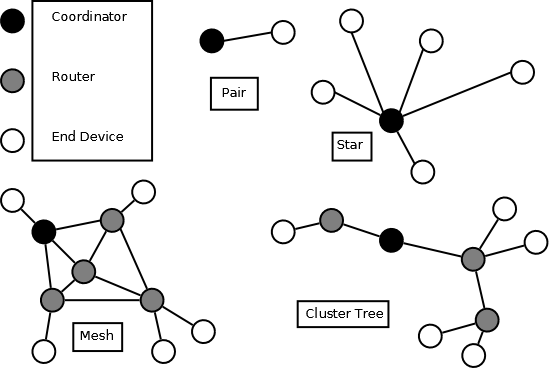
\includegraphics[scale=0.3]{Hardware/images/ZigBeeNetworkTypes.png}
\caption{ZigBee Network Topologies}
\label{NetTopo}
\end{figure}
\subsection{Potential Problems}
XBee Series 2 radios and their interface boards have as of yet been unexplored. 
This means that as with the rest of this project, there will be about as much learning as there will be doing. 
To counteract this somewhat, the engineers in charge of weaving the Mesh have learning materials that are perfect for this project. 
\newpage
\section{Logging In}

In this scenario the user logs into the system.

\subsubsection{Actors}
\begin{itemize}
	\item User
	\item System
\end{itemize}

\subsubsection{Assumptions}

The user has valid login information\\
The user has the login page open in their browser

\subsubsection{Procedure}

The system prompts the user for a username and password\\
The user enters their username and password\\
The user clicks a "OK" or "Submit" button\\
The system logs the user in

\subsubsection{Expected Outcome}

The user is now logged in.
\newpage
\section{Logging Out}
In this scenario the user logs out of the system.

\subsubsection{Actors}
\begin{itemize}
	\item User
	\item System
\end{itemize}

%This is a bulleted list of the actors

\subsubsection{Assumptions}

The user is logged in\\
The user is on any page

\subsubsection{Procedure}

The user clicks the logout button\\
The system logs the user out\\
The display informs the user that they have been logged out\\
The system returns the user to the login page

\subsubsection{Expected Outcome}

The user is now logged out.
\newpage
\section{View Monthly Power Consumption}
In this scenario the user is intending to view the power consumption of the entire house for a series of specified consecutive months.

\subsubsection{Actors}
\begin{itemize}
	\item User
	\item Display
	\item System
\end{itemize}


\subsubsection{Assumptions}

The user is logged into the display site\\
The user is at the home page\\
The system has logged data from at least one month ago 

\subsubsection{Procedure}

The user clicks the "View Data" button in the navigation menu\\
The display opens a drop-down menu with several more links
\begin{itemize}
	\item One of which is "View Device Power Consumption" 
\end{itemize}
The user selects "View Device Power Consumption"\\
The user specifies the date range that will viewed\\
The user clicks a "OK" or "Submit" button\\
The display shows the user a table containing:
\begin{itemize}
	\item The name of the month
	\item The total power consumed by the entire system for that month 
\end{itemize}
The site displays the sum of the power consumption for each Satellite on each day of the month 

\subsubsection{Expected Outcome}

The site will display the power consumption from the specified month or a warning if the data does not exist.
\newpage
\section{View Largest Power Consumer}
This use case describes the process that a user would employ to display a list of the largest power consumers being recorded by the system.
\subsubsection{Actors}
\begin{itemize}
	\item User
	\item Display
\end{itemize}

\subsubsection{Assumptions}

The user is logged in and on the home page\\
There are several devices associated with the server 

\subsubsection{Procedure}

The user clicks the "View Data" button from the navigation menu\\
The display opens a drop-down menu with several more links
\begin{itemize}
	\item One of which is "Device Power Consumption" 
\end{itemize}
The user selects "Device Power Consumption"\\
The display shows the user a table containing:
\begin{itemize}
	\item The name of each device
	\item The power consumed by each device
	\item The device's power consumption per hour
	\item Sorted alphabetically by name 
\end{itemize}
The user clicks on the "Power consumed" column to sort it from greatest to least\\
The display sorts the list from greatest power consumption to least

\subsubsection{Expected Outcome}

The user sees that the first item in the list is using the most power.\\
The user sees the next few largest power-consuming devices.
\newpage
\section{View Power Consumption Over Time}
This use case describes the process that a user would employ to display graphs indicating the power consumption of devices over a specified time range.

\subsubsection{Actors}
\begin{itemize}
	\item User
	\item Display
\end{itemize}

\subsubsection{Assumptions}

The user is logged in and on the home page\\
There are several devices associated with the server\\
The server has several months worth of data 

\subsubsection{Procedure}

The user selected the "View Data" button from the navigation menu\\
The display shows the user a list of charts they can view
\begin{itemize}
	\item One of which is "View Power Use over Time" 
\end{itemize}
The display shows a page that prompts the user to select:
\begin{itemize}
	\item What devices or device groups they want to compare
	\begin{itemize}
		\item Defaults the group "All devices" 
	\end{itemize}
	\item What time period they would like to compare them over
	\begin{itemize}
		\item Defaults to the last six months 
	\end{itemize}
\end{itemize}
The user supplies the requested information
The user clicks "Display"
The display generates one chart for each device/device group over the specified range
Displays them in the order the user selected them 

\subsubsection{Expected Outcome}

The user sees the power consumption trends of the selected devices over the selected time period 
\newpage
\section{Adjust Power Cost}
This use case describes the process that a user would employ to change the cost-per-kilowatt-hour that the system uses to guesstimate the monthly power bill.

\subsubsection{Actors}
\begin{itemize}
	\item User
	\item Display
\end{itemize}

\subsubsection{Assumptions}

The user is logged in and on the home page\\
The user has permission to change the kilowatt\/hr cost 

\subsubsection{Procedure}

The user clicks the "Settings" link from the navigation menu\\
The display presents the user with the settings panel, which includes a link to the "Adjust Power Cost" page\\
The user clicks the "Adjust Power Cost" link\\
The display presents the user with a page consisting of two columns of text boxes. The left column indicates the range for the cost, which is specified in the right column\\
\begin{itemize}
	\item The goal is to allow the user to say "My first 500 kW/hrs cost \$0.08, my next 1000 kW/hrs cost \$0.10, and everything after that costs \$0.12 per kW\/hr" 
\end{itemize}
The user adjusts the cost by changing the ranges or changing the costs\\
The user clicks a "Submit" button\\
The display shows the changed power costs

\subsubsection{Expected Outcome}

The display applies the changed power costs to all new calculations. 
Previous calculations shall remain unchanged, with assumption that costs just increased.
\newpage
\section{Add User}

This use case documents the procedure that a user would use to add a new user.

\subsubsection{Actors}
\begin{itemize}
	\item User
	\item Display
\end{itemize}

\subsubsection{Assumptions}

The user is logged in and on the home page\\
The user has permission to modify user permissions

\subsubsection{Procedure}

The user clicks the "Settings" link from the navigation menu\\
The display presents the user with the settings panel, which includes a link to the "User Management" page\\
The user clicks the "User Management" link\\
The display shows the user the "User Management" page
\begin{itemize}
	\item This includes a button to add a user 
\end{itemize}
The user clicks "Add user"\\
The display presents the user with a page that contains the necessary fields to create a new user:
\begin{itemize}
	\item First Name
	\item Last Name
	\item Username
	\item Password
	\item A check-box requiring the user to change their password at login
	\item A multi-select to put them into groups
	\item A list of permissions to give the user 
\end{itemize}
The user supplies the requested information\\
The user clicks a "Submit" button \\
The display informs the user that the user has been added\\
The display shows the user the "User Management" page

\subsubsection{Expected Outcome}

A new user was added with the requested username, password, and permissions.
\newpage
\section{Delete User}

This use case documents the procedure that a user would use to delete a user.

\subsubsection{Actors}
\begin{itemize}
	\item User
	\item Display
\end{itemize}

\subsubsection{Assumptions}

The user is logged in and on the home page\\
The user has permission to modify user permissions

\subsubsection{Procedure}

The user clicks the "Settings" link from the navigation menu\\
The display presents the user with the settings panel, which includes a link to the "User Management" page\\
The user clicks the "User Management" link\\
The display shows the user the "User Management" page
\begin{itemize}
	\item This includes a button to delete a user
\end{itemize}
The display presents the user with a list of users with check-boxes next to their usernames\\
The user then clicks on the check-box next to appropriate username\\
The user clicks "Delete user" \\
The display shows a dialog box asking to confirm the delete\\
The user clicks on "Apply action" \\
The display informs the user that the user has been deleted\\
The display shows the user the "User Management" page\\

\subsubsection{Expected Outcome}

A user was deleted from the system by another authorized user.
\newpage
\section{Add Device}

This use case documents the procedure that a user would use to add a new device to the system. 

\subsubsection{Actors}
\begin{itemize}
	\item User
	\item Display
	\item Device
\end{itemize}

\subsubsection{Assumptions}

The user is logged in and on the home page\\
The user has permission to modify devices

\subsubsection{Procedure}

The user clicks the "Settings" link from the navigation menu\\
The display presents the user with the settings panel, which includes a link to the "Device Management" page\\
The user clicks the "Device Management" link\\
The display shows the user the "Device Management" page
\begin{itemize}
	\item This includes an "Add device" button
\end{itemize}
The user clicks the "Add device" button\\
The display prompts the user for information about the device, including:
\begin{itemize}
	\item Name
	\begin{itemize}
		\item Optional: room, location in room, owner. These will be used to guide the user in coming up with a unique name
	\end{itemization}
	\item What Satellite it is plugged into
	\begin{itemization}
		\item Optional, may be not be plugged in
	\end{itemization}
\end{itemize}
The user fills in the requested information\\
The user clicks an "OK" or "Submit" button\\
The display informs the user that the device has been added\\
The display shows the user the "Device Management" page

\subsubsection{Expected Outcome}

The display has the device available for history and mapping to Satellites. 
\newpage
\section{Rename Device}

This use case documents the procedure that a user would use to rename a device associated with an outlet.

\subsubsection{Actors}
\begin{itemize}
	\item User
	\item Display
	\item Device
\end{itemize}

\subsubsection{Assumptions}

The user is logged in and on the home page\\
The user has permission to modify outlet-device mappings 

\subsubsection{Procedure}

The user clicks the "Settings" link from the navigation menu\\
The display presents the user with the settings panel, which includes a link to the "Device Management" page\\
The user clicks the "Device Management" link\\
The display shows the user the "Device Management" page
\begin{itemize}
	\item This includes a list of all existing devices 
\end{itemize}
The user clicks on the row of the device they want to edit\\
The display presents a page with a form that allows the user to edit the name of the device\\
The user changes the name of the device\\
The user clicks "Submit" or "Save" \\
The display informs the user that the device has been renamed\\
The display shows the user the "User Management" page

\subsubsection{Expected Outcome}

The device is now know by a new name.
\newpage
\section{Disable Device}

This use case documents the procedure that a user would use to disable a device.

\subsubsection{Actors}
\begin{itemize}
	\item User
	\item Display
	\item Device
\end{itemize}

\subsubsection{Assumptions}

The user is logged in and on the home page\\
The user has permission to modify devices

\subsubsection{Procedure}

The user clicks the "Settings" link from the navigation menu\\
The display presents the user with the settings panel, which includes a link to the "Device Management" page\\
The user clicks the "Device Management" link
\begin{itemize}
	\item This includes a drop down with an action to disable a device
	\item This includes a table listing all the devices, with check-boxes next to each row
\end{itemize}
The user selects the 'Disable Device" action\\
The user then clicks on the check-boxes next to appropriate devices\\
The user clicks an "OK" or "Submit" or "Apply" button\\
The display shows a dialog box asking to confirm applying the action\\
The user clicks on "Apply action" \\
The display informs the user that the device has been disabled\\
The display shows the user the "Device Management" page\\

\subsubsection{Expected Outcome}

A device was disabled and will no longer appear in any menus.
\newpage
\section{Re-enable Device}

This use case documents the procedure that a user would use to re-enable a device.

\subsubsection{Actors}
\begin{itemize}
	\item User
	\item Display
	\item Device
\end{itemize}

\subsubsection{Assumptions}

The user is logged in and on the home page\\
The user has permission to modify devices

\subsubsection{Procedure}

The user clicks the "Settings" link from the navigation menu\\
The display presents the user with the settings panel, which includes a link to the "Device Management" page\\
The user clicks the "Device Management" link\\
The display shows the user the "Device Management" page
\begin{itemize}
	\item This includes a link to a "Disabled device Management" page
\end{itemize}
The user clicks on the "Disabled device Management" link\\
The display shows the user the "Disabled device Management" page
\begin{itemize}
	\item This includes a drop down with an action to re-enable a device
	\item This includes a table listing all the devices, with check-boxes next to each row
\end{itemize}
The user selects the "Re-enable Device" action\\
The user then clicks on the check-boxes next to appropriate devices\\
The user clicks an "OK" or "Submit" or "Apply" button\\
The display shows a dialog box asking to confirm applying the action\\
The user clicks on "Apply action" \\
The display informs the user that the device has been re-enabled\\
The display shows the user the "Device Management" page

\subsubsection{Expected Outcome}

A disabled device was re-enabled and will appear in all menus.
\newpage
\section{Remap Device}

This use case documents the procedure that a user would use to associate a device with a Satellite.

\subsubsection{Actors}
\begin{itemize}
	\item User
	\item Display
	\item Satellite
\end{itemize}

\subsubsection{Assumptions}

The user is logged in and on the home page\\
The user has permission to modify Satellites and modify devices\\
The device has been created\\
The Satellite has been associated with the display

\subsubsection{Procedure}

The user clicks the "Settings" link from the navigation menu\\
The display presents the user with the settings panel, which includes a link to the "Device Management" page\\
The user clicks the " Device Management" link\\
The display shows the user the " Device Management" page
\begin{itemize}
	\item This includes a table listing all the Satellites
\end{itemize}
The user clicks on the row of the device they wish to associate with a Satellite\\
The display shows the user a page that contains information about the selected device
\begin{itemize}
	\item Including a drop down that allows the user to select the associated Satellite
\end{itemize}
The user selects the Satellite the device is plugged into from the drop down\\
The user clicks a "OK" or "Submit" button\\
The display informs the user that device has been updated\\
The display shows the user the "Device Management" page

\subsubsection{Expected Outcome}

The device has been associated with a new Satellite, and all data from that Satellite will be attributed to the specified device.
\newpage
\section{Adding a Satellite}

This use case documents the procedure that a user would use to associate a new Satellite with the display.

\subsubsection{Actors}
\begin{itemize}
	\item User
	\item Display
	\item Satellite
\end{itemize}

\subsubsection{Assumptions}

The user is logged in and on the home page\\
The user has permission to modify Satellites\\
The user has plugged the Satellite into the wall\\
Everything goes according to plan

\subsubsection{Procedure}

The user clicks the "Settings" link from the navigation menu\\
The display presents the user with the settings panel, which includes a link to the "Satellite Management" page\\
The user clicks the "Satellite Management" link\\
The display shows the user the "Satellite Management" page
\begin{itemize}
	\item This includes an "Add Satellite" button
\end{itemize}
The user clicks the "Add Satellite" button\\
The display prompts the user to press the "Connect" button on the Satellite and then click "OK"\\
The user presses the "Connect" button on the Satellite\\
The display informs the user that it's searching\\
The display then displays the serial number (xxx-xxx) of the connected Satellite\\
The user confirms that this is the correct Satellite\\
The display shall informs the user that a new Satellite was connected\\
The display shows the user the "Satellite Management" page

\subsubsection{Expected Outcome}

A new Satellite was added to the display.
\newpage
\section{Removing a Satellite}

This use case documents the procedure that a user would use to remove a Satellite with the display.

\subsubsection{Actors}
\begin{itemize}
	\item User
	\item Display
	\item Satellite
\end{itemize}

\subsubsection{Assumptions}

The user is logged in and on the home page\\
The user has permission to modify Satellites\\
The Satellites being removed do not have any devices associated with them

\subsubsection{Procedure}

The user clicks the "Settings" link from the navigation menu\\
The display presents the user with the settings panel, which includes a link to the "Satellite Management" page\\
The user clicks the "Satellite Management" link\\
The display shows the user the "Satellite Management" page
\begin{itemize}
	\item This includes a drop down with an action to remove Satellites
	\item This includes a table listing all the Satellites, with check-boxes next to each row
\end{itemize}
The user clicks on the appropriate check-boxes next to the Satellites\\
The user selects the "Remove Satellite" action from the drop down menu\\
The user clicks "Apply" or "OK"\\
The display prompts user to confirm the removal\\
The user clicks "Submit" or "OK"\\
The display informs the user that the Satellites were removed\\
The display shows the user the "Satellite Management" page

\subsubsection{Expected Outcome}

The specified Satellites have been removed from the display. 
No historical data should have been lost due to this procedure.
\newpage

% Stuff about the server
%% Template file for all Software/Hardware modules

% Replace "Name of Module" with the name of this module
\chapter{Hardware Design Overview}

\section{Description}

The POW-R project is comprised of two main hardware components, the Server and the Satellites. 
The Server refers to the physical hardware from which the Display shall be served. 
It also acts as the data center for all Satellites associated to it, collecting data and storing it in a hard drive. 
The Satellites will talk over ZigBee specification to the one Zigbee module connected to the Server. 
That one Zigbee module can talk to the Server over Universal Serial Bus (USB).
 
Figure \ref{SystemOverview} shows the layout of the hardware system.

\begin{figure}[H]
\centering
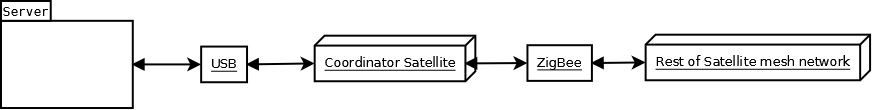
\includegraphics[scale=0.3]{Hardware/images/SystemOverview.png}
\caption{System Overview}
\label{SystemOverview}
\end{figure}

\section{The Server}
%% Template file for all Hardware modules

% Replace "Name of Module" with the name of this module
\subsection{PC Hardware}

\subsubsection{Mainboard}
The Server's main hardware component is the mainboard, a SYS9400-ECX Developer-Ready Reference Platform. 
It's a small form-factor, low-power machine with the following specs:

\begin{itemize}
	\item 1.6 GHz Intel Atom E6XX Series Processor
	\item 1 GB DDR2 RAM
	\item Roughly 6" by 4"
	\item Various connection interfaces:
	\begin{itemize}
		\item 2x SATA ports
		\item Header for Solid State Drive (SSD) power
		\item Ethernet port
		\item 5x USB 2.0 ports
		\item General Purpose Input/Output (GPIO) pin header
	\end{itemize}
\end{itemize}

\subsubsection{Potential Problems}
If for whatever reason using this mainboard falls through: 
It should be noted that the requirements for the Server hardware concern not just specifications, but interfaces as well.
In particular, this project requires at least Ethernet, 2 USB ports, a SATA port, and accessible GPIO pins.
\subsubsection{Storage}
The Server's mainboard is connected via SATA to a 40GB SSD.

\subsubsection{Power Supply}
An adapter rated for 12VDC @ 3A is used to connect the Server's board to mains electricity.

%% Template file for all Software/Hardware modules

\subsection{Add-Ons}
The Server provides for the computational needs of the POW-R project; 
More hardware shall be added before the utility needs of the project are met.

\subsubsection{IP Display}
The IP of the Server shall be displayed somewhere on it's casing. 
The user will enter this IP into their browser to access the Display.

This will be achieved by connecting an Arduino via USB to the Server, and housing it inside the Server's casing. 
The Arduino will be connected to an LCD display which will output the network IP of the Server. 
Figure \ref{ArduinoLCD} shows the interaction between Server and Arduino.

\begin{figure}
\centering
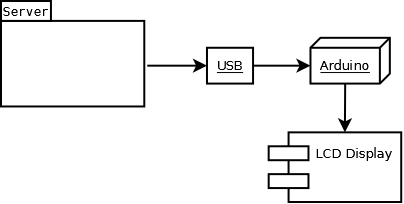
\includegraphics[scale=0.5]{Hardware/images/ArduinoLCD.png}
\caption{IP Display Diagram}
\label{ArduinoLCD}
\end{figure}

The IP of the system can be obtained via kernel module, and sent to the Arduino one byte at a time. 
This works well, since the Arduino connects over serial and thusly takes a byte at a time.

\subsection{GPIO Pins}
As mentioned above in the "PC Hardware" section, the mainboard is outfitted with a GPIO pin header. 
A Linux distribution will be used for the Server's operating system, which must support interaction with such pins. 

A folder can be found in the Linux kernel, at the location \filename{/sys/class/gpio} that helps with GPIO manipulation. 
To set up a single GPIO pin, one must type the following command into a terminal (as root):

\begin{lstlisting}
	$ echo N > /sys/class/gpio/export
	(where N must be a GPIO pin number)
\end{lstlisting}

When this command is issued, a directory is made inside the \filename{gpio} directory, named \filename{gpioN}, where N is the GPIO pin number you passed. 
Two files will be in that new directory, \filename{direction} and \filename{value}. 
\filename{direction} can only contain "in" or "out" with no leading characters, spaces, line breaks, etc.
\filename{value} can only contain "1" or "0" and can be read or written to at any time.
These files, \filename{direction} and \filename{value} are responsible for what kind of pin it is (input or output) and what the current value is (1 or 0), respectively.

NOTE: The pin number you must echo into \filename{/sys/class/gpio/export} is not necessarily the number of the actual pin on the board, but may refer to the pin of the bridge that connects the GPIO port to the motherboard.

The subsections below are buttons that the Server must have, and each of these buttons connects to a GPIO pin.


\subsubsection{Power Switch}
A standard rocker switch will be added to the case to provide the user with a way to turn the Server on and off. 
The style of the switch will clearly signify "On" or "Off".

\subsubsection{Factory Reset\repeatfootnote{opt}}
This button should intentionally be placed somewhere inconvenient: 
Sunken into the case far enough that you need a skinny rod (such as a paperclip) to push it, and in a spot
that chaotic forces (children, mean people, God's divine will) will not notice it.

\subsubsection{Connect to Satellite}
A button will be added to the Server that allows a user to add a Satellite easily.
When a user wants to add a Satellite to the network, the following series of events should take place, in order:

\begin{itemize}
	\item User plugs Satellite into wall outlet
	\item User presses "connect" button on Satellite
	\item User presses "connect" button on Server
	\item Satellite is now connected
\end{itemize}
	
\subsection{Server Hull}
The Server needs a protective casing, for several reasons. 
On the physical level, a durable casing will protect the hardware. 
The casing also serves to render unnecessary ports inaccessible to users. 
Lastly, the casing is important in the sense that the term "Server" currently only applies to the mainboard, 
and most people think of a legitimate Server as something physical, encased in a box, that's protected and hidden away, exactly as a Server should be.

As far as prototyping goes, the casing can be as simple as a folded piece of aluminum
with holes cut in it to fit the IP display, the buttons, and any ports that must be
exposed. As an end-game product, the casing would probably be a little less "junkyard."

\input{Hardware/Server-TalkToXbee}
\subsection{Potential Problems}
As of right now, the Server has not been explored, and as with the rest of this project, is unfamiliar territory. 


\section{The Satellites}
The Satellites are made up of two sets of hardware: 
Instruments for measuring current and voltage, and radios for communicating that data to the Server. 
The end product shall have a hard casing around it, NEMA 5-15 sockets on one side, and prongs for a NEMA 5-15 male end on the other. 
However, it should be noted that prototyping will most likely involve all of the hardware being spread out on breadboards.
%% Template file for all Software/Hardware modules

% Replace "Name of Module" with the name of this module
\subsection{Measurement Hardware}
Current and voltage running through the mains outlet to the Satellite's associated device must be measured and sent to the Server. 

%% Template file for all Software/Hardware modules

\subsection{Communications Hardware}

% Describe hardware setup for our
% XBee modules

For the communication between the Server and the Satellites,
we will be using the Xbee Series 2 Radio Modules.

\subsubsection{XBee Series 2 Radio Modules}

% Might want to mention we want series 2 for
% Zigbee, but ZigBee has it's own module since
% it's a fairly large part of this design

\subsubsection{Interface Board}

% This section is a little vague at the moment.
% Currently we're using Digi Interface Boards,
% but we may need to move to an Arduino if these
% boards lack an A/D converter pin. Haven't
% looked into it yet. In either case, whatever
% interface board we use will connect the
% measuring circuit to the radio. Might
% need diagram for this.

%% Template file for all Software/Hardware modules

\subsection{ZigBee Standard}
ZigBee is a standard that uses 802.15.4 wireless protocol as it's foundation. It's 
particularly useful for setting up ad-hoc mesh networks. Much like how any Bluetooth
devices can talk to each other, any ZigBee devices nearby can talk to each other (so 
long as they have the proper permissions).

\subsubsection{Why ZigBee?}
The advantage of using ZigBee is that it lines up with the requirements of the POW-R
project. It's a specification targeted for low-power, low-data applications that need
to be secure. 

Another advantage of using ZigBee is that XBee radios, which also fit the requirements
of the POW-R project, are ZigBee-compliant, so the forming of a mesh network can happen
quickly and easily.

\subsubsection{Device Types}
The nodes of a ZigBee network are obviously ZigBee devices, but from the network's
perspective, there are three distinct types of ZigBee device:

\begin{itemize}
	\item Coordinator
	\item Router
	\item End Device
\end{itemize}

The coordinator runs the network, keeps it healthy, makes sure everybody is talking when
they should be, and overall, just maintains the Mesh. It is also the device that is 
typically plugged into a computer via USB or some other serial interface, meaning
that this is the node you want to send data to. There cannot be a ZigBee network
without exactly one coordinator.

Routers are fully functional ZigBee modules, capable of taking care of themselves and
routing messages across the Mesh. Routers are capable of being "parent" devices.

End devices are low-power ZigBee devices that don't do any routing. They can only talk
to one other device, which is referred to as it's "parent" device. A router or a coordinator
may be a parent device, but not another end device.

In the POW-R project, the coordinator will be attached to the Server so that it may
also act as a data bridge between the Server and the Satellites. The rest of the 
Satellites are routers; There will be no end devices in the POW-R's mesh network.


\subsubsection{Network Topology}
Zigbee supports four network topologies, shown in Figure \ref{NetTopo}. A ZigBee network
is defined by two rules:

\begin{itemize}
	\item A ZigBee network must have two or more ZigBee devices
	\item One of those devices \emph{must} be a coordinator
\end{itemize}

As mentioned before, the POW-R project will use the Mesh configuration, but without end 
devices. This means that the Mesh will consist entirely of routers and one coordinator.

\begin{figure}
\centering
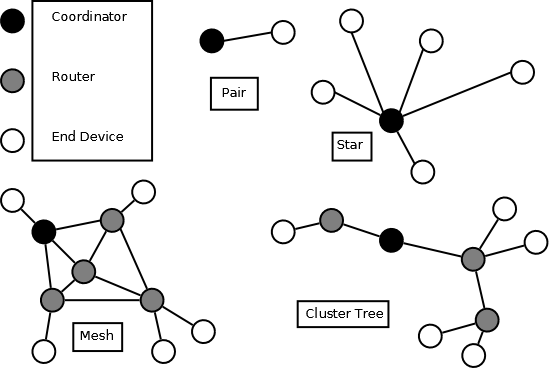
\includegraphics[scale=0.3]{Hardware/images/ZigBeeNetworkTypes.png}
\caption{ZigBee Network Topologies}
\label{NetTopo}
\end{figure}
\subsection{Potential Problems}
XBee Series 2 radios and their interface boards have as of yet been unexplored. 
This means that as with the rest of this project, there will be about as much learning as there will be doing. 
To counteract this somewhat, the engineers in charge of weaving the Mesh have learning materials that are perfect for this project. 

\section{Acronyms}
\begin{acronym}
	\acro{A}{Amps}
	\acro{AJAX}{Asynchronous JavaScript and XML}
	\acro{API}{Application programming interface}
	\acro{CSS}{Cascading Style Sheets}
	\acro{GPIO}{General Purpose Input Output}
	\acro{HTML}{HyperText Markup Language}
	\acro{HTTP}{Hypertext Transfer Protocol}
	\acro{IEEE}{Institute of Electrical and Electronics Engineers}
	\acro{IP}{Internat Protocol}
	\acro{JSON}{JavaScript Object Notation}
	\acro{LCD}{Liquid Crystal Display}
	\acro{M}{Meters}
	\acro{NEMA}{National Electrical Manufacturers Association}
	\acro{PIP}{Python package installer}
	\acro{POST}{Request Method}
	\acro{POW-R}{Power Outlet Wireless Reporter}
	\acro{REST}{REpresentational State Transfer}
	\acro{SATA}{Serial ATA}
	\acro{SQL}{Structured Query Language}
	\acro{SSD}{Solid State Srive}
	\acro{TLS}{Transport Layer Security}
	\acro{UI}{User Interface}
	\acro{URL}{Uniform Resource Locator}
	\acro{USB}{Universal Serial Bus}
	\acro{VDC}{Volts DC (Direct Current)}
	\acro{W}{Watts}
	\acro{XML}{Extensible Markup Language}
	\acro{XSS}{Cross-site scripting}
	\acro{YAML}{YAML Ain't Markup Language}
\end{acronym}
\newpage

% References
\bibliographystyle{plain}
\bibliography{biblo}

\end{document}